\documentclass[a4paper]{article}
\usepackage[a4paper,margin=0mm]{geometry}
\usepackage{fontspec}
\usepackage{unicode-math}
\usepackage{tikz}
\usetikzlibrary{fit,calc,positioning}
\usepackage[table]{xcolor}
\usepackage[absolute]{textpos}
\usepackage{array}

\setmainfont{Libertinus Serif}
\setsansfont{Libertinus Sans}
\setmathfont{Libertinus Math}

\definecolor{accent}{HTML}{F46530}
\definecolor{badge}{HTML}{FFBDA5}
\definecolor{ink}{HTML}{2A2E30}

\setlength{\TPHorizModule}{1mm}
\setlength{\TPVertModule}{1mm}
\setlength{\parindent}{0pt}
\pagestyle{empty}

\newcommand{\topicheader}[2]{%
\begin{textblock*}{194mm}(16mm,10mm)
\begin{tikzpicture}
\node[fill=accent,text=white,font=\sffamily\bfseries\fontsize{13}{13}\selectfont,
      minimum width=9mm,minimum height=9mm,inner sep=0pt] at (4.5mm,-4.5mm) {#1};
\node[font=\sffamily\bfseries\fontsize{15}{16}\selectfont,text=ink,anchor=west] at (12mm,-4.5mm) {#2};
\end{tikzpicture}
\end{textblock*}
\begin{textblock*}{194mm}(16mm,22.5mm)

\begin{tikzpicture}
\fill[accent] (0,0) rectangle (194mm,0.5mm);
\end{tikzpicture}
\end{textblock*}
}

\newcommand{\pagekicker}[1]{%
\begin{textblock*}{100mm}(16mm,25.5mm)
\begin{tikzpicture}
\node[fill=ink,text=white,font=\sffamily\bfseries\fontsize{8}{8}\selectfont,
      inner sep=2.2pt,rounded corners=1pt] {\MakeUppercase{#1}};
\end{tikzpicture}
\end{textblock*}
}

\newcommand{\pagefooter}[1]{%
\begin{textblock*}{194mm}(8mm,286.41mm)
  
\begin{tikzpicture}
    \fill[accent] (0,0) rectangle (194mm,0.6mm);
  \end{tikzpicture}
\end{textblock*}
\begin{textblock*}{63.59mm}(8mm,288.27mm)
  {\sffamily\bfseries\color{accent}\fontsize{13}{16}\selectfont SAT 1200+}
\end{textblock*}
\begin{textblock*}{10mm}(188mm,288.27mm)
  \centering{\sffamily\color{accent}\fontsize{14}{16}\selectfont #1}
\end{textblock*}
}

\newcommand{\cardbg}[4]{%
\begin{textblock*}{#3mm}(#1mm,#2mm)
\begin{tikzpicture}
\fill[badge!22,rounded corners=3mm] (0,0) rectangle (#3mm,-#4mm);
\end{tikzpicture}
\end{textblock*}%
}

\newcommand{\pill}[3]{%
\begin{textblock*}{160mm}(#1mm,#2mm)
\begin{tikzpicture}
\node[fill=accent,text=white,anchor=north west,font=\sffamily\bfseries\fontsize{10}{10}\selectfont,
      rounded corners=8pt,inner xsep=5mm,inner ysep=1.8mm] at (0,0) {QOIDA ~\textperiodcentered~ #3};
\end{tikzpicture}
\end{textblock*}%
}

\arrayrulecolor{accent}
\setlength{\arrayrulewidth}{0.7pt}
\renewcommand{\arraystretch}{1.5}

\begin{document}

\topicheader{7}{Darajalar va ildizlar}
\pagekicker{Formula sheet}
\pagefooter{55}
\mbox{}%

% ================= CARD 1: Bir xil asosli daraja qoidalari (y: 33-91) =================
\cardbg{16}{33}{178}{58}
\pill{26}{36}{Bir xil asosli daraja qoidalari}

\begin{textblock*}{158mm}(26mm,47mm)
{\fontsize{11}{14}\selectfont
\begin{tabular}{|>{\centering\arraybackslash}p{60mm}|>{\centering\arraybackslash}p{80mm}|}
\hline
\rowcolor{accent}
{\color{white}\textbf{Qoida}} & {\color{white}\textbf{Misol}} \\ \hline
$a^m\times a^n=a^{m+n}$ & $2^3\times2^4=2^{3+4}=2^7$ \\ \hline
$(a^m)^n=a^{mn}$ & $(2^7)^2=2^{7\times2}=2^{14}$ \\ \hline
$\dfrac{a^m}{a^n}=a^{m-n}$ & $\dfrac{2^{14}}{2^5}=2^{14-5}=2^9$ \\ \hline
\end{tabular}}
\end{textblock*}

% ================= CARD 2: Nol va manfiy daraja (y: 97-172) =================
\cardbg{16}{97}{178}{75}
\pill{26}{100}{Nol va manfiy daraja}

\begin{textblock*}{158mm}(26mm,111mm)
{\fontsize{11}{14}\selectfont\color{ink}
Nolmas $a$ uchun: $a^0=1$. Manfiy ko'rsatkich -- teskari sonni bildiradi, asosni manfiy qilmaydi:}
\end{textblock*}

\begin{textblock*}{158mm}(26mm,124mm)
\begin{tikzpicture}[every node/.style={font=\fontsize{15}{15}\selectfont}]
\node[anchor=west] (l0) at (0,0) {$5^0+2^{-3}\times4^2$};
\node[anchor=west,font=\sffamily\bfseries\scriptsize,text=accent] at (62mm,0) {$\leftarrow$ 1. $a^0{=}1$,\ $a^{-n}{=}\frac{1}{a^n}$};

\node[anchor=west] (l1) at (0,-18mm) {$1+\dfrac{1}{8}\times16$};
\node[anchor=west,font=\sffamily\bfseries\scriptsize,text=accent] at (62mm,-18mm) {$\leftarrow$ 2. ko'paytiring};

\node[anchor=west] (l2) at (0,-36mm) {$1+2$};
\node[anchor=west,font=\sffamily\bfseries\fontsize{16}{16}\selectfont,text=accent] at (40mm,-36mm) {$=3$};

\foreach \y in {-5,-23}{
  \draw[accent,->,line width=1pt] (6mm,\y mm) -- (6mm,\y mm -6mm);
}
\end{tikzpicture}
\end{textblock*}

% ================= CARD 3: Kvadrat ildizni soddalashtirish (y: 178-253) =================
\cardbg{16}{178}{178}{75}
\pill{26}{181}{Kvadrat ildizni soddalashtirish}

\begin{textblock*}{158mm}(26mm,192mm)
{\fontsize{11}{14}\selectfont\color{ink}
Eng katta to'liq kvadrat ko'paytuvchini toping, so'ng ajrating: $\sqrt{ab}=\sqrt{a}\times\sqrt{b}$.}
\end{textblock*}

\begin{textblock*}{158mm}(26mm,205mm)
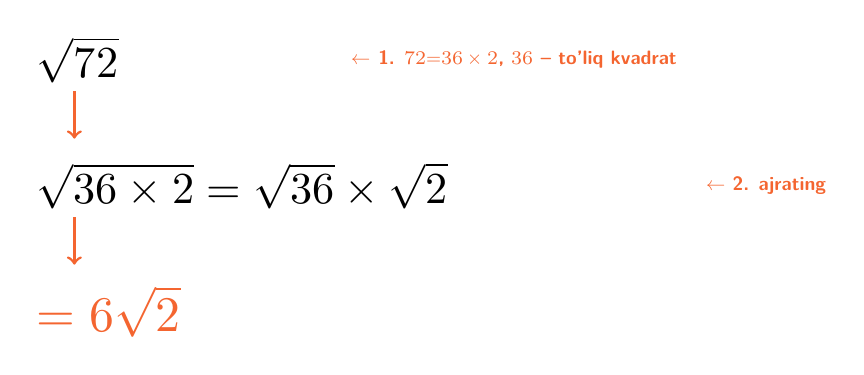
\begin{tikzpicture}[every node/.style={font=\fontsize{16}{16}\selectfont}]
\node[anchor=west] (l0) at (0,0) {$\sqrt{72}$};
\node[anchor=west,font=\sffamily\bfseries\scriptsize,text=accent] at (40mm,0) {$\leftarrow$ 1. $72{=}36\times2$,\ $36$ -- to'liq kvadrat};

\node[anchor=west] (l1) at (0,-16mm) {$\sqrt{36\times2}=\sqrt{36}\times\sqrt{2}$};
\node[anchor=west,font=\sffamily\bfseries\scriptsize,text=accent] at (85mm,-16mm) {$\leftarrow$ 2. ajrating};

\node[anchor=west,font=\sffamily\bfseries\fontsize{18}{18}\selectfont,text=accent] (l2) at (0,-32mm) {$=6\sqrt{2}$};

\foreach \y in {-4,-20}{
  \draw[accent,->,line width=1pt] (6mm,\y mm) -- (6mm,\y mm -6mm);
}
\end{tikzpicture}
\end{textblock*}

\begin{textblock*}{158mm}(26mm,245mm)
{\fontsize{9}{11}\selectfont\color{black!55}\itshape Eslatma: $\sqrt{a+b}\neq\sqrt{a}+\sqrt{b}$ -- masalan $\sqrt{16+9}=5$, biroq $\sqrt{16}+\sqrt{9}=7$.}
\end{textblock*}

\end{document}
